\documentclass[conference]{IEEEtran}

\usepackage[utf8]{inputenc}
\usepackage[T1]{fontenc}
\usepackage[spanish,es-nodecimaldot]{babel}
\usepackage{cite}
\usepackage{amsmath,amssymb}
\usepackage{graphicx}
\usepackage{booktabs}
\usepackage{tabularx}
\usepackage{array}
\usepackage{xcolor}
\usepackage{url}
\usepackage[hidelinks]{hyperref}
\usepackage{siunitx}
\usepackage{microtype}

\graphicspath{{figuras/}}
\sisetup{output-decimal-marker={,}}

\newcommand{\evidencia}[1]{%
  \begin{center}
  \fcolorbox{gray}{gray!8}{%
    \parbox{0.91\columnwidth}{\centering\small
    \textbf{Evidencia pendiente:} #1}}
  \end{center}}

\newcommand{\figpendiente}[2]{%
  \begin{figure}[!t]
    \centering
    \fbox{\parbox[c][3.2cm][c]{0.92\columnwidth}{%
      \centering\small\textit{Insertar: #1}}}
    \caption{#2}
    \label{fig:#1}
  \end{figure}}

\newcommand{\imgslot}[1]{%
  \fbox{\parbox[c][2.35cm][c]{0.93\linewidth}{%
    \centering\small\textit{#1}}}}

\title{SmartSense Monitoring: Sistema Inalámbrico para el Monitoreo y Análisis Histórico de Temperatura en Equipos Industriales}

\author{
\IEEEauthorblockN{Jesus Andre Bojaca Lopez y David Santiago Puentes Cárdenas}
\IEEEauthorblockA{
Programa de Ingeniería Electrónica, Facultad de Ingeniería\\
Universidad ECCI, Bogotá D.C., Colombia\\
\{jesusa.bojacal, davids.puentesc\}@ecci.edu.co}
}

\begin{document}

\maketitle

\begin{abstract}
Este artículo presenta el diseño, implementación y evaluación preliminar de SmartSense Monitoring, un sistema inalámbrico para medir temperatura superficial en equipos de una planta piloto. La solución está compuesta por nodos con microcontrolador XIAO ESP32-C6, sondas PT100 de tres hilos, acondicionadores MAX31865, alimentación mediante batería y comunicación LoRa con módulos Ebyte E220. Un gateway con ESP32-C6 recibe las mediciones, las almacena en una tarjeta microSD y las presenta mediante una pantalla local y un dashboard web. A diferencia de una inspección manual puntual, la solución conserva el comportamiento térmico durante las 24 horas, permite consultar días anteriores, comparar sensores, aplicar compensaciones de temperatura y configurar alarmas. Durante la validación en planta, el histórico permitió observar un incremento de temperatura en el motor de un succionador después de la parada de la máquina; el comportamiento se relacionó posteriormente con una condición anómala de los rodamientos. El sistema se comparó cualitativamente con una pistola de temperatura Fluke y con un sensor Advantech WISE-2410 en la configuración disponible en planta. Los resultados funcionales verificaron la adquisición, transmisión, almacenamiento, visualización histórica, compensación y gestión de alarmas. La evaluación cuantitativa de exactitud y disponibilidad se completará con los registros pareados de los instrumentos de referencia.
\end{abstract}

\begin{IEEEkeywords}
Internet de las cosas industrial, LoRa, PT100, MAX31865, monitoreo de temperatura, mantenimiento predictivo, dashboard, ESP32-C6.
\end{IEEEkeywords}

\section{Introducción}

El seguimiento de temperatura en motores y otros equipos industriales permite identificar cambios asociados con fricción, sobrecarga, ventilación deficiente o degradación mecánica. En una inspección manual, el operario obtiene únicamente el valor correspondiente al instante de la medición. Si este valor no se registra de manera sistemática, no es posible reconstruir la evolución térmica del equipo ni relacionarla con sus ciclos de operación y parada.

Las redes de sensores inalámbricos permiten distribuir puntos de medición sin instalar cableado de comunicación en cada ubicación \cite{akyildiz2002,yick2008}. Para aplicaciones de baja tasa de datos, LoRa ofrece una alternativa de largo alcance y bajo consumo adecuada para nodos alimentados por batería \cite{centenaro2016,semtech2015}. Estas características se aprovecharon en SmartSense Monitoring para construir una plataforma local, modular y configurable.

El propósito del proyecto fue implementar y validar un sistema capaz de medir temperatura superficial, transmitirla de manera inalámbrica, conservar un histórico por sensor y facilitar el análisis del comportamiento térmico. El trabajo evolucionó desde un anteproyecto hasta un prototipo funcional instalado en una planta piloto. Por tanto, este documento describe las actividades realizadas y los resultados evidenciados, en lugar de presentar únicamente resultados esperados.

Las contribuciones principales del proyecto fueron: 1) integración de nodos PT100 de tres hilos con comunicación LoRa; 2) almacenamiento diario con respaldo local; 3) dashboard de 24 horas con comparación de sensores; 4) compensación configurable de temperatura; y 5) alarmas térmicas visuales, sonoras y mediante salida física.

\section{Arquitectura del sistema}

La arquitectura implementada, mostrada conceptualmente en la Fig.~\ref{fig:arquitectura}, está formada por nodos sensores, un enlace LoRa, un gateway y clientes locales conectados por Wi-Fi. Cada nodo adquiere la temperatura y el estado estimado de batería. El gateway recibe las tramas, identifica el nodo, aplica la compensación configurada, almacena la muestra y actualiza la interfaz.

\begin{figure*}[!t]
  \centering
  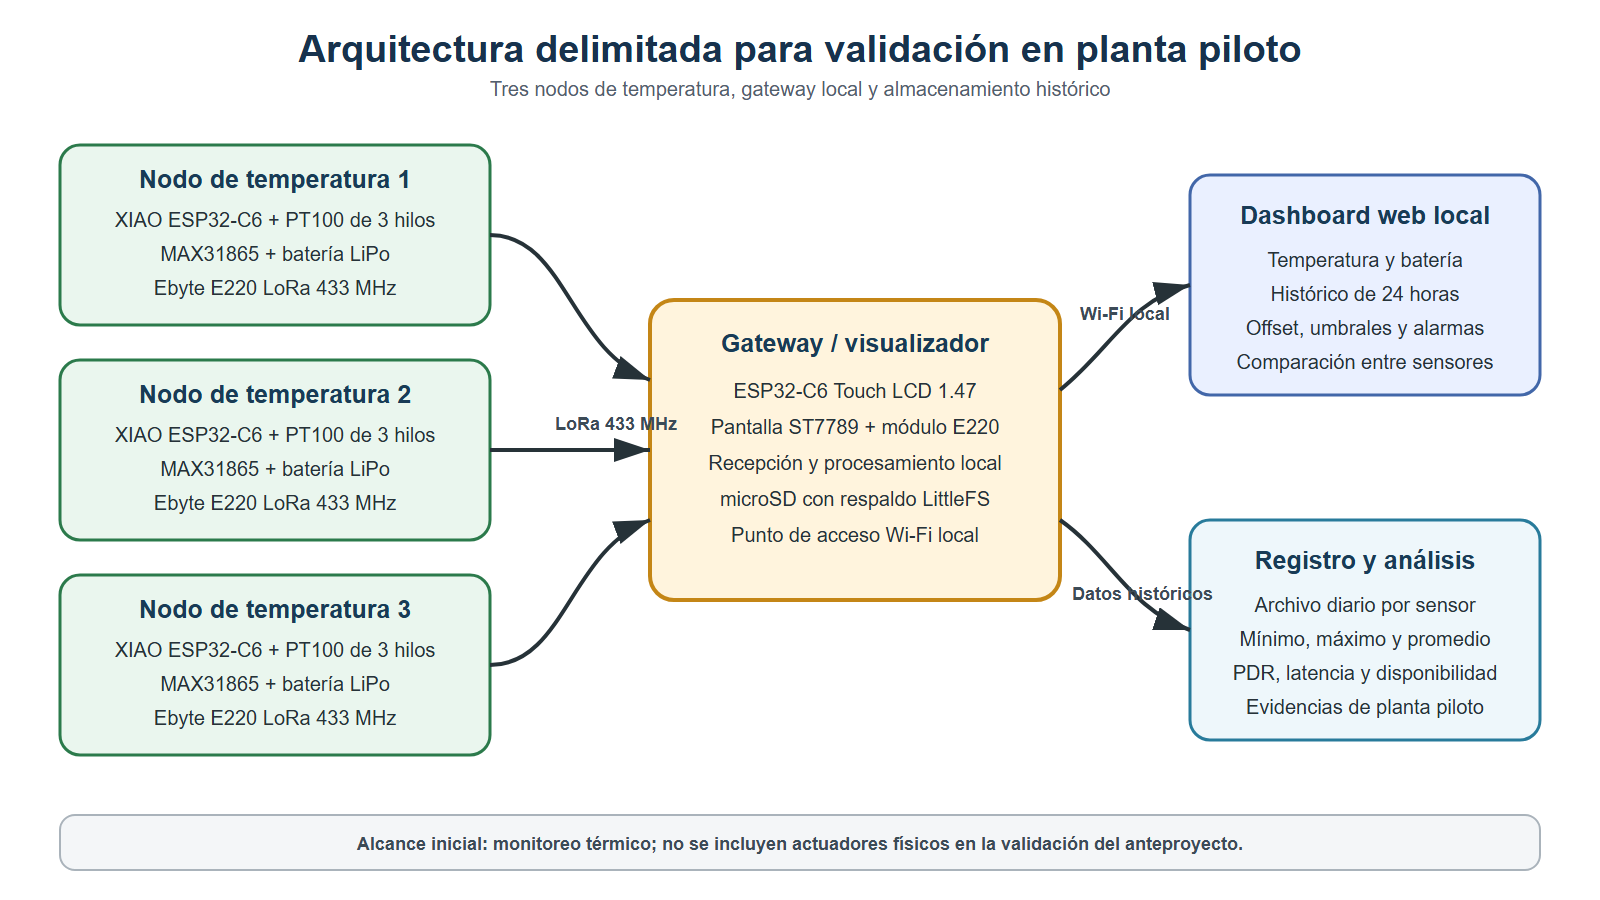
\includegraphics[width=0.9\textwidth]{arquitectura_smartsense.png}
  \caption{Arquitectura implementada de SmartSense Monitoring: nodos de temperatura con XIAO ESP32-C6, PT100 y MAX31865, enlace LoRa de 433~MHz, gateway/visualizador con pantalla táctil y almacenamiento local, dashboard web servido por Wi-Fi local y registro histórico para análisis.}
  \label{fig:arquitectura}
\end{figure*}

\subsection{Nodo sensor}

Cada nodo fue construido con un Seeed Studio XIAO ESP32-C6, una sonda PT100 de tres hilos, un MAX31865, una batería LiPo y un módulo Ebyte E220. El MAX31865 fue configurado mediante la biblioteca de Adafruit en el modo \texttt{MAX31865\_3WIRE}. Se utilizó una resistencia nominal de \SI{100}{\ohm} y una resistencia de referencia caracterizada en \SI{421.1}{\ohm}.

En cada ciclo se efectuaron varias conversiones de temperatura y se descartaron valores inválidos. El firmware también consultó el registro de fallas del MAX31865 para detectar problemas de conexión o lecturas fuera de rango. La tensión de batería se obtuvo mediante el convertidor analógico-digital del ESP32-C6 y un divisor resistivo. El porcentaje estimado se calculó entre \SI{3.30}{\volt} y \SI{4.10}{\volt}.

La trama de aplicación incluyó el identificador del nodo, temperatura, porcentaje de batería y dirección MAC. Después de la transmisión, el nodo ingresó en sueño profundo. El periodo puede configurarse entre 5 y 7200 segundos; durante la versión evaluada se utilizó un valor predeterminado de 60 segundos.

La Fig.~\ref{fig:esquematico-nodo} presenta el esquemático de conexiones del nodo: la interfaz SPI hacia el MAX31865, el enlace UART hacia el módulo E220, la alimentación del acondicionador conmutada por un pin digital para reducir el consumo durante el sueño profundo, y el divisor resistivo utilizado para estimar la carga de la batería.

\begin{figure*}[!t]
  \centering
  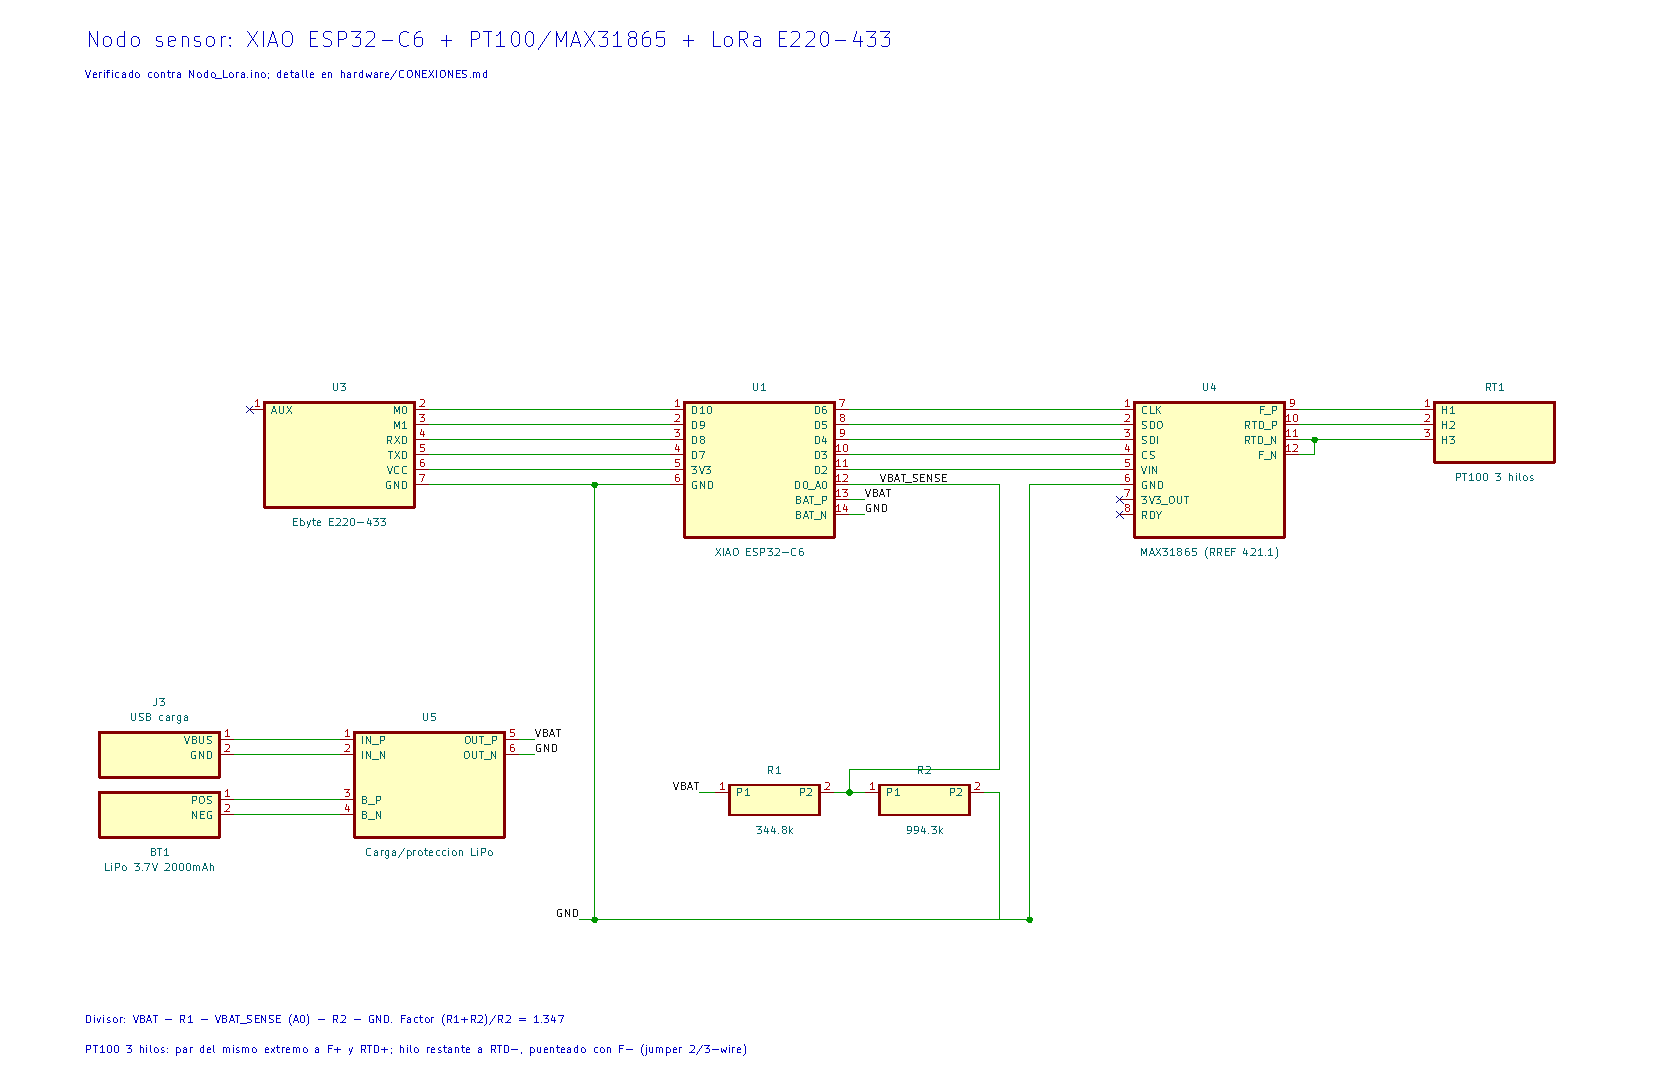
\includegraphics[width=\textwidth]{esquematico-nodo.pdf}
  \caption{Esquemático de conexiones del nodo sensor: XIAO ESP32-C6, acondicionador MAX31865 con sonda PT100 de tres hilos, módulo LoRa Ebyte E220-433, circuito de carga y divisor resistivo para la estimación de batería. Los saltos largos se indican con etiquetas de red (VBAT, GND, VBAT\_SENSE).}
  \label{fig:esquematico-nodo}
\end{figure*}

\subsection{Comunicación LoRa}

La comunicación se implementó con módulos UART Ebyte E220 configurados mediante comandos AT. Se utilizó direccionamiento fijo, un canal común para los nodos y el gateway, velocidad serial de 9600 bit/s y velocidad aérea de 2,4 kbit/s. La dirección MAC identifica de manera persistente cada sensor, mientras que la dirección de radio permite encaminar los mensajes.

El firmware del gateway posee un campo reservado para RSSI, pero la versión revisada no habilita ni procesa dicho valor desde el E220. Tampoco se procesa la relación señal-ruido (SNR). En consecuencia, estas variables no se presentan como resultados experimentales del prototipo actual.

\subsection{Gateway y persistencia}

El gateway fue implementado con un ESP32-C6, pantalla táctil con controlador ST7789, módulo E220 y tarjeta microSD. La tarjeta se utiliza como medio principal para los históricos. Si no está disponible, LittleFS funciona como respaldo.

Para cada dirección MAC se crea un directorio independiente y un archivo por fecha. Cada línea contiene el segundo transcurrido desde el inicio del día y la temperatura representada con resolución de \SI{0.1}{\celsius}. El firmware conserva hasta 30 días por sensor. La hora se sincroniza desde el navegador y se ajusta a la zona horaria UTC--5, por lo cual el sistema puede trabajar localmente sin conexión permanente a Internet.

La Fig.~\ref{fig:esquematico-gateway} resume las conexiones externas del gateway. La pantalla, el panel táctil y la ranura microSD están integrados en la placa; las conexiones agregadas corresponden al módulo E220 por UART, con las líneas de modo M0 y M1 unidas a un mismo pin, y a la salida digital para la señalización de alarma crítica.

\begin{figure*}[!t]
  \centering
  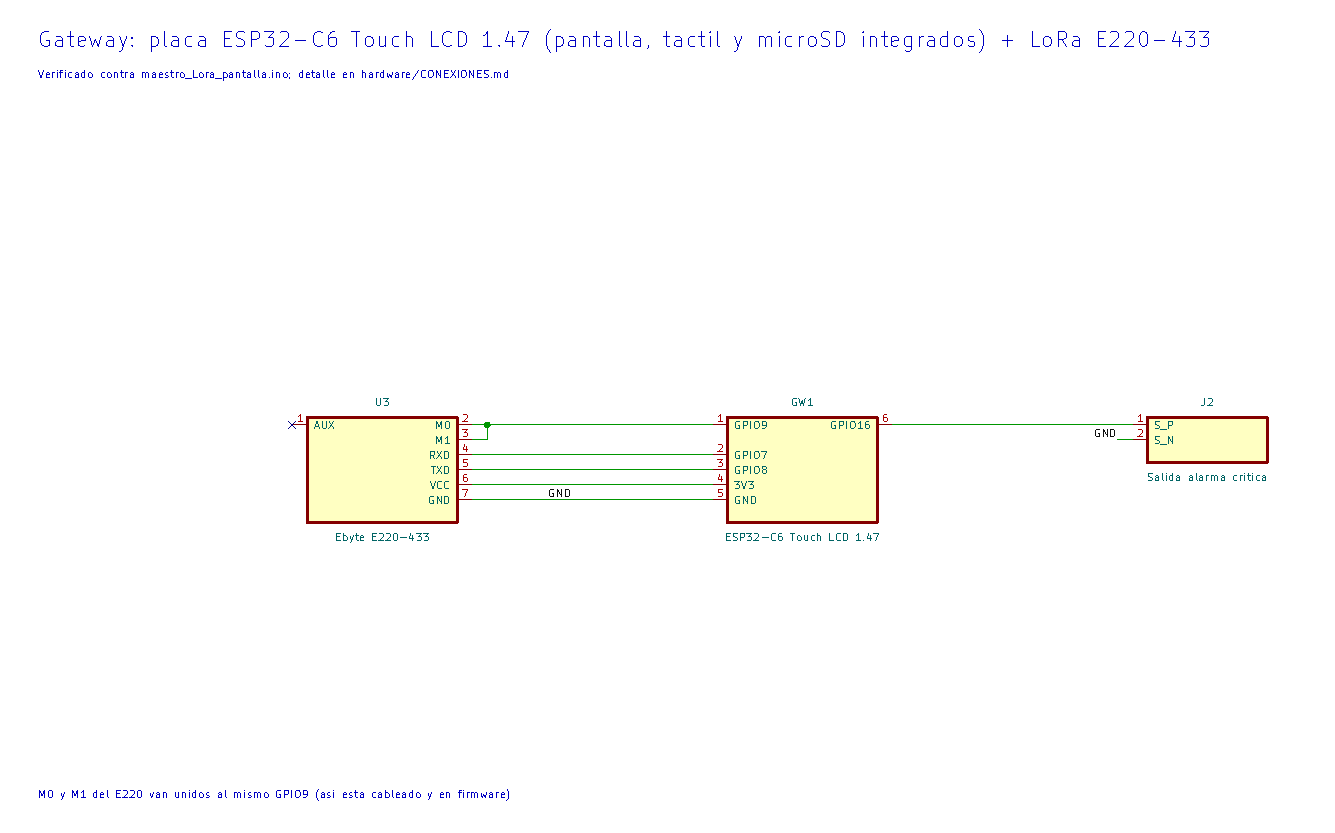
\includegraphics[width=0.85\textwidth]{esquematico-gateway.pdf}
  \caption{Esquemático de conexiones externas del gateway/visualizador: placa ESP32-C6 con pantalla táctil, módulo LoRa Ebyte E220-433 y salida de alarma crítica.}
  \label{fig:esquematico-gateway}
\end{figure*}

\section{Dashboard y funciones de supervisión}

El gateway crea el punto de acceso Wi-Fi \texttt{Sensores\_Temp} y publica el dashboard en la dirección local \texttt{192.168.4.1}. La actualización de los datos se realiza mediante eventos enviados por el servidor aproximadamente cada segundo.

La interfaz implementada permite visualizar temperatura, batería y conectividad; consultar fechas disponibles; representar las 24 horas; obtener mínimo, máximo y promedio; comparar sensores de una misma máquina; asignar nombres; configurar el intervalo de muestreo; aplicar compensaciones; y establecer umbrales de advertencia y condición crítica.

La Fig.~\ref{fig:dashboard-principal} muestra nueve sensores registrados y organizados en cinco grupos: Twin, Molino 1, Empaque A, Cuarto Frío y sensores aún sin asignar. Cada tarjeta presenta la última temperatura, batería, estado de conexión, intervalo térmico y una minigráfica. La agrupación permite comparar sensores pertenecientes a una misma máquina y reduce el tiempo necesario para localizar una condición anómala. La interfaz también integra accesos a emergencias, configuración y selección del diseño visual.

\begin{figure*}[!t]
  \centering
  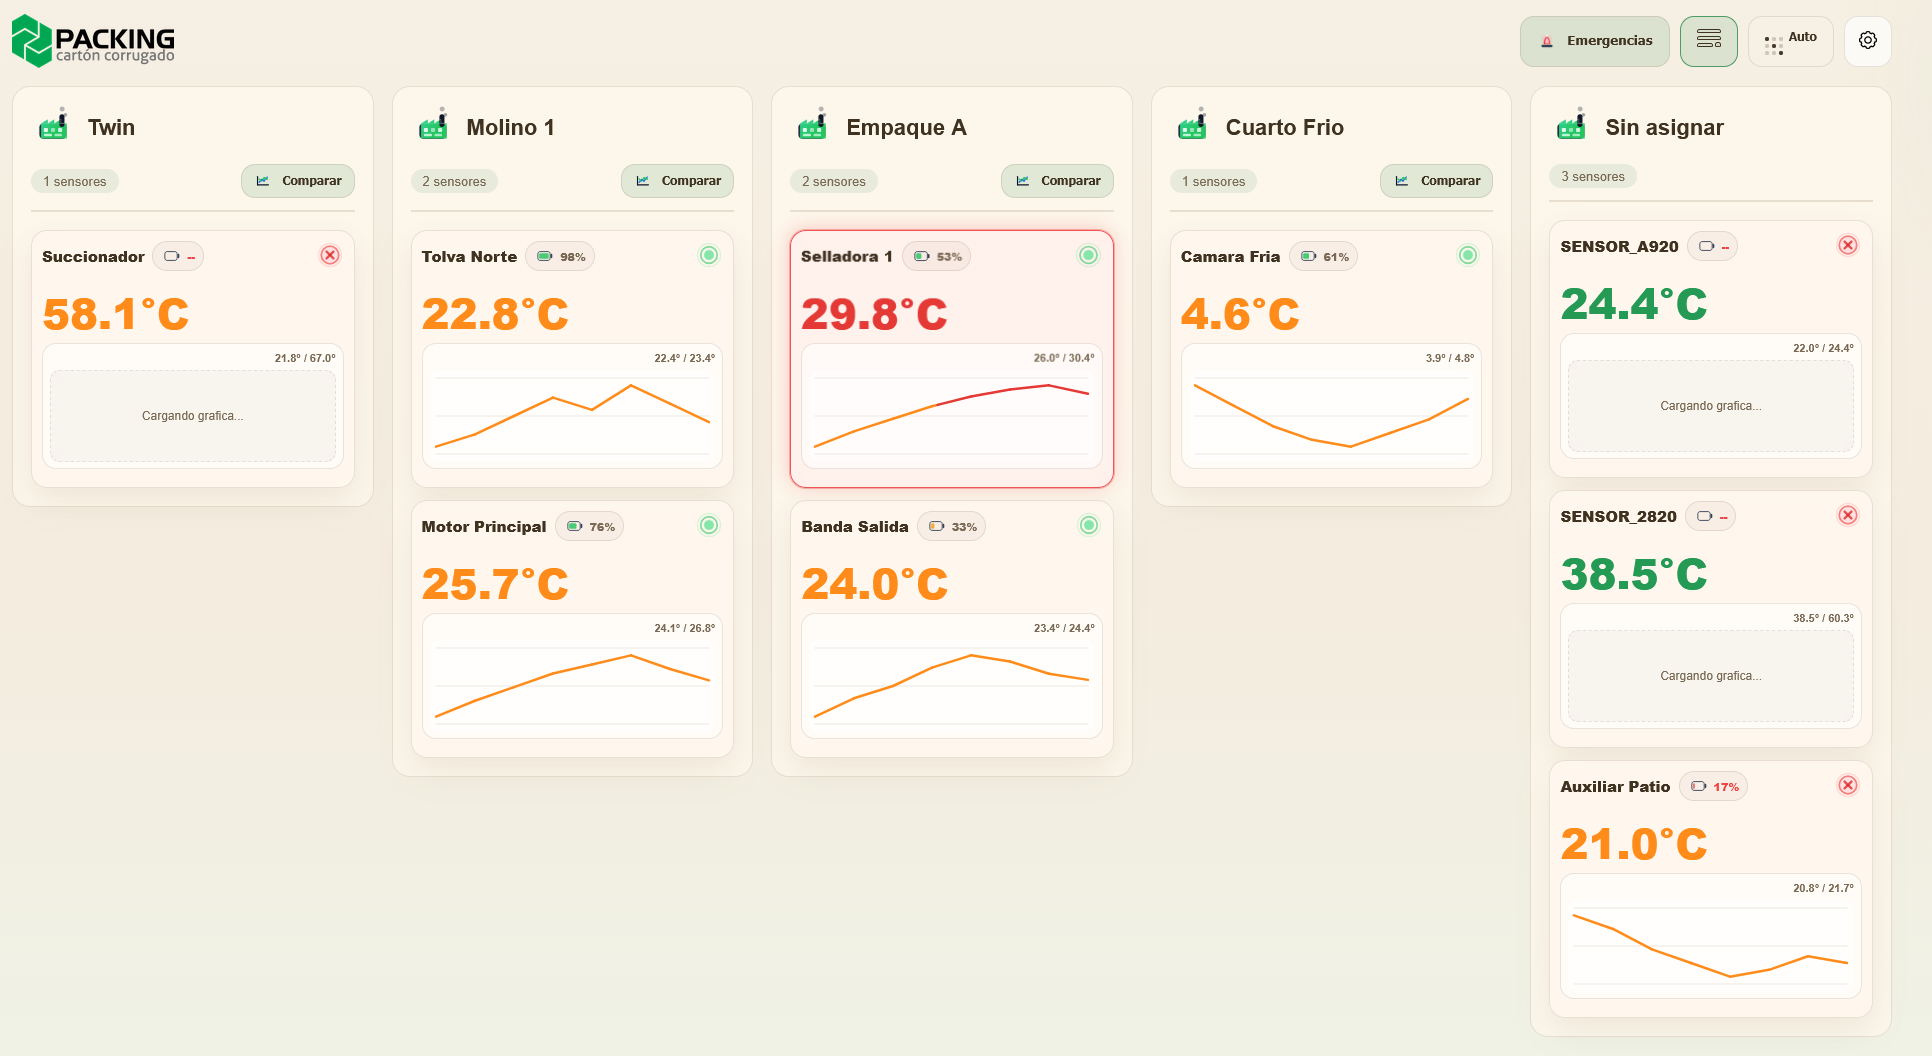
\includegraphics[width=\textwidth]{dashboard-principal.png}
  \caption{Interfaz principal de SmartSense Monitoring con los sensores agrupados por máquina. La captura evidencia la supervisión simultánea de nueve registros y la presentación de temperatura, batería, conectividad y tendencia reciente.}
  \label{fig:dashboard-principal}
\end{figure*}

\subsection{Compensación de temperatura}

Para aproximar la lectura de cada PT100 al instrumento de referencia se implementó una compensación configurable. El usuario captura una referencia en condición fría y posteriormente establece un ajuste en condición caliente. Entre ambos puntos, el firmware aplica una compensación progresiva.

Si $T_r$ es la temperatura cruda, $T_f$ la referencia fría, $T_c$ el punto de calibración caliente y $O$ el offset establecido, la compensación dentro del intervalo puede expresarse como

\begin{equation}
T_{corr}=T_r+O\left(\frac{T_r-T_f}{T_c-T_f}\right),
\label{eq:offset}
\end{equation}

limitando el factor de interpolación entre cero y uno. Por debajo de la referencia fría no se aplica corrección y, por encima del punto caliente, se aplica el offset completo.

\evidencia{tabla con lectura cruda, cámara termográfica, offset y lectura corregida para cada nodo.}

\subsection{Alarmas}

Cada nodo posee un umbral de advertencia y un umbral crítico configurables. Al superar el primero, el dashboard cambia la representación visual. Al superar el segundo, se activa el estado crítico, una alarma sonora opcional en el navegador y la salida física definida en el gateway. El usuario puede silenciar la alarma sin eliminar el registro del evento.

La arquitectura permite integrar posteriormente módulos de relés o variables de control. Sin embargo, cualquier acción automática sobre maquinaria debe diferenciarse de las alarmas ya verificadas y validarse bajo criterios de seguridad industrial.

\section{Metodología de evaluación}

La validación se estructuró en cuatro etapas. Primero se verificó la lectura de las PT100 y el reporte de fallas del MAX31865. Luego se comprobó el envío de tramas y la identificación de los nodos. En la tercera etapa se validaron el almacenamiento, la consulta por fecha y las funciones del dashboard. Finalmente, el sistema se instaló temporalmente en equipos de la planta para observar el comportamiento térmico durante la operación.

La exactitud se evaluará con muestras pareadas entre SmartSense y un instrumento de referencia. Para $n$ pares de datos, el error absoluto medio se calcula mediante

\begin{equation}
\mathrm{MAE}=\frac{1}{n}\sum_{i=1}^{n}\left|T_{SS,i}-T_{ref,i}\right|.
\label{eq:mae}
\end{equation}

También se calcularán temperatura mínima, máxima, promedio, diferencia antes y después del offset y duración de los incrementos térmicos relevantes.

\begin{table}[!t]
\caption{Formato de medición pareada en planta}
\label{tab:mediciones}
\centering
\footnotesize
\begin{tabular}{@{}lccc@{}}
\toprule
Hora & SmartSense & Referencia & Estado \\
 & (\si{\celsius}) & (\si{\celsius}) & máquina \\
\midrule
Pendiente & -- & -- & Operación/parada \\
Pendiente & -- & -- & Operación/parada \\
Pendiente & -- & -- & Operación/parada \\
\bottomrule
\end{tabular}
\end{table}

\section{Comparación con métodos disponibles}

\subsection{Medición manual con pistola Fluke}

En el primer escenario, un operario se desplaza hasta el equipo y obtiene una lectura puntual. Por ejemplo, una medición de \SI{60}{\celsius} en el motor del succionador describe únicamente el instante de la inspección. El procedimiento resulta útil como verificación directa, pero depende de la disponibilidad del operario y no conserva automáticamente la evolución anterior y posterior.

\subsection{Advantech WISE-2410}

El WISE-2410 disponible en la planta es un dispositivo industrial de monitoreo de condición que integra acelerómetro de tres ejes, temperatura, procesamiento local y LoRaWAN \cite{wise2410}. Su capacidad de medir vibración constituye una ventaja para el diagnóstico mecánico.

La comparación de visualización se restringió a la configuración y plataforma disponibles en la planta. En esta implementación, el equipo de trabajo observó una ventana temporal limitada y no dispuso de la misma flexibilidad para ajustar la lectura térmica o consultar directamente un día completo. Esta observación no se presenta como una limitación general del WISE-2410, pues sus capacidades dependen del gateway, servidor y aplicación empleados.

\subsection{SmartSense Monitoring}

SmartSense presentó el historial de la fecha seleccionada sobre un eje de 24 horas, compensación independiente por nodo, comparación entre sensores y umbrales configurables. Además, funcionó mediante una red local sin depender de servicios externos.

\begin{table*}[!t]
\caption{Comparación cualitativa de los métodos evaluados}
\label{tab:comparacion}
\centering
\footnotesize
\begin{tabularx}{\textwidth}{@{}p{2.8cm}XXX@{}}
\toprule
\textbf{Criterio} & \textbf{Pistola Fluke} & \textbf{WISE-2410 evaluado} & \textbf{SmartSense Monitoring} \\
\midrule
Adquisición & Puntual y manual & Automática y periódica & Automática y periódica \\
Dependencia del operario & Alta & Baja & Baja \\
Histórico & Requiere registro externo & Depende de la plataforma instalada & Archivo diario por sensor \\
Visualización observada & Un valor instantáneo & Ventana disponible en planta & Fecha seleccionable y 24 horas \\
Ajuste térmico & Depende del instrumento & No disponible para el equipo en la interfaz evaluada & Offset configurable por nodo \\
Alarmas & No incorporadas & Dependen de la integración & Advertencia, crítica, visual y sonora \\
Comparación entre sensores & No & Depende de la plataforma & Incluida en el dashboard \\
Variables & Temperatura & Vibración y temperatura & Temperatura, batería, conexión y alarmas \\
Operación sin Internet & Sí & Depende de la arquitectura & Sí, mediante servidor local \\
\bottomrule
\end{tabularx}
\end{table*}

\section{Resultados obtenidos}

La Tabla~\ref{tab:resultados} resume las funciones verificadas mediante revisión del firmware y pruebas funcionales del prototipo. Los resultados cuantitativos de planta se mantienen separados hasta incorporar los archivos originales y las mediciones de referencia.

\begin{table}[!t]
\caption{Resultados funcionales verificados}
\label{tab:resultados}
\centering
\footnotesize
\begin{tabularx}{\columnwidth}{@{}Xc@{}}
\toprule
\textbf{Función} & \textbf{Estado} \\
\midrule
Lectura de PT100 de tres hilos & Implementada \\
Detección de fallas del MAX31865 & Implementada \\
Identificación individual de nodos & Implementada \\
Temperatura y batería en la trama & Implementada \\
Sueño profundo y periodo configurable & Implementada \\
Almacenamiento microSD/LittleFS & Implementada \\
Histórico por sensor y fecha & Implementada \\
Gráfica diaria de 24 horas & Implementada \\
Mínimo, máximo y promedio & Implementada \\
Comparación de sensores & Implementada \\
Offset progresivo por nodo & Implementada \\
Umbrales y alarmas & Implementada \\
Exportación directa CSV & Por verificar \\
RSSI y SNR experimentales & No implementados \\
\bottomrule
\end{tabularx}
\end{table}

\subsection{Despliegue de 32 días y disponibilidad}

Se analizó un registro real de la planta con \num{51338} muestras provenientes de tres nodos, con un intervalo de muestreo mediano de \SI{121}{\second}. La Fig.~\ref{fig:val-serie} presenta la serie completa de temperatura de uno de los nodos durante el despliegue, en la que se aprecia el máximo de \SI{70.0}{\celsius} asociado al caso del succionador.

La Fig.~\ref{fig:val-cobertura} muestra la cobertura de datos de los tres nodos. Las interrupciones no se distribuyen de forma independiente entre nodos, sino que ocurren de manera \emph{simultánea} en los tres, con el mismo instante de inicio. Este comportamiento indica que las interrupciones no correspondieron a fallas del enlace LoRa —que afectarían a un nodo a la vez— sino a periodos en los que el gateway permaneció apagado durante paradas de planta y de energía.

En consecuencia, la Tabla~\ref{tab:disponibilidad} reporta dos indicadores. La disponibilidad cruda considera todo el intervalo de despliegue, incluidos los periodos de gateway apagado. La disponibilidad del enlace excluye dichos periodos, identificados por su simultaneidad, y estima la fracción de tramas efectivamente recibidas mientras el sistema estuvo activo. La disponibilidad del enlace se mantuvo por encima del \SI{97}{\percent} en los tres nodos. La Fig.~\ref{fig:val-intervalos} confirma la regularidad de la recepción durante los tramos activos: la mayoría de los intervalos entre llegadas se concentraron alrededor de la mediana de \SI{121}{\second}.

\begin{figure}[!t]
  \centering
  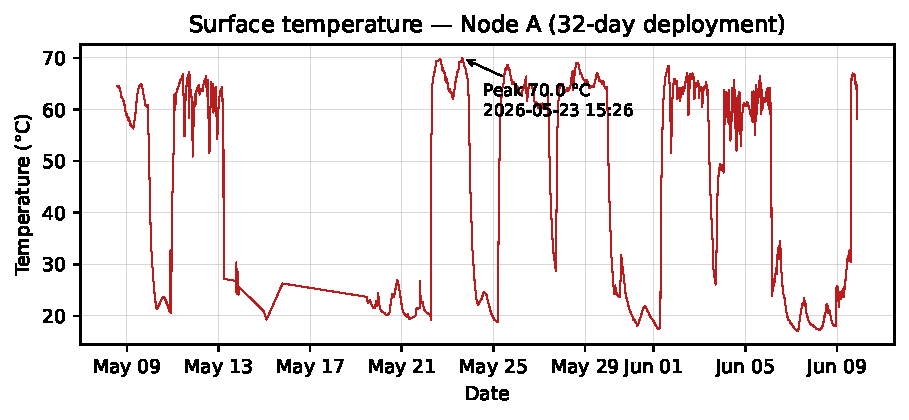
\includegraphics[width=\columnwidth]{val-serie-evento.pdf}
  \caption{Serie de temperatura superficial de un nodo durante el despliegue de 32 días, con el máximo asociado al caso del succionador.}
  \label{fig:val-serie}
\end{figure}

\begin{figure}[!t]
  \centering
  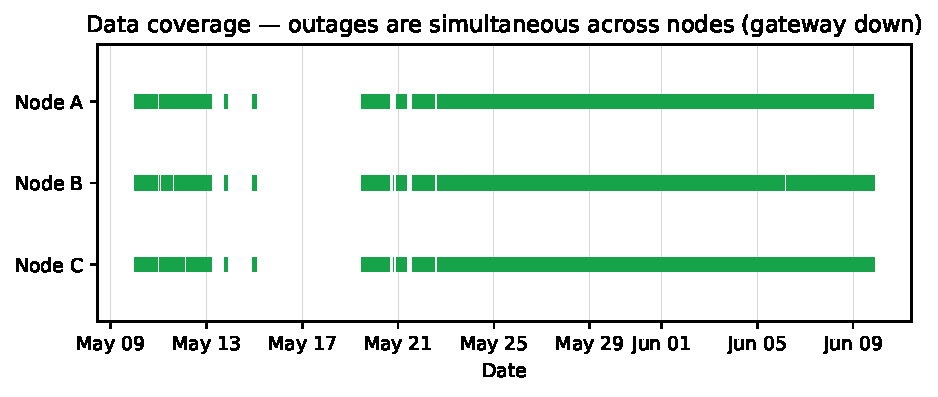
\includegraphics[width=\columnwidth]{val-cobertura.pdf}
  \caption{Cobertura de datos de los tres nodos. Las interrupciones son simultáneas en todos los nodos, lo que corresponde a periodos de gateway apagado (paradas de planta) y no a fallas del enlace LoRa.}
  \label{fig:val-cobertura}
\end{figure}

\begin{table}[!t]
\caption{Disponibilidad por nodo durante el despliegue}
\label{tab:disponibilidad}
\centering
\footnotesize
\begin{tabularx}{\columnwidth}{@{}Xccccc@{}}
\toprule
\textbf{Nodo} & \textbf{Muestras} & \textbf{Cruda} & \textbf{Enlace} & \textbf{Paradas} & \textbf{h fuera} \\
\midrule
Nodo A & \num{17537} & \SI{76.0}{\percent} & \SI{98.4}{\percent} & 66 & 176 \\
Nodo B & \num{16487} & \SI{32.3}{\percent} & \SI{98.3}{\percent} & 73 & 1154 \\
Nodo C & \num{17314} & \SI{75.1}{\percent} & \SI{97.8}{\percent} & 81 & 180 \\
\bottomrule
\end{tabularx}
\vskip 0.2cm
{\footnotesize La disponibilidad del enlace excluye los periodos de gateway apagado, identificados por ser simultáneos en los tres nodos. El Nodo B incluye una parada prolongada de aproximadamente 33 días.}
\end{table}

\begin{figure}[!t]
  \centering
  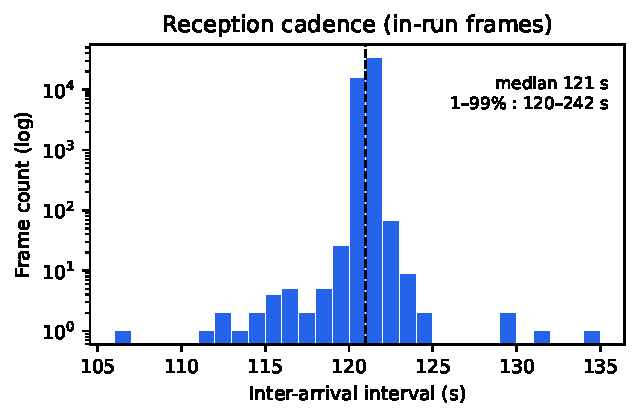
\includegraphics[width=0.75\columnwidth]{val-intervalos.pdf}
  \caption{Distribución de los intervalos entre llegadas durante los tramos activos. La escala vertical es logarítmica; la mayoría de las tramas se recibieron con una cadencia cercana a la mediana de \SI{121}{\second}.}
  \label{fig:val-intervalos}
\end{figure}

\subsection{Caso del motor del succionador}

La Fig.~\ref{fig:historico-succionador} corresponde al succionador de la máquina Twin y presenta una jornada completa, desde aproximadamente las 00:01 hasta las 23:59. Al inicio se observó una condición relativamente estable cercana a \SIrange{48}{49}{\celsius}. Alrededor de la 01:30 ocurrió un incremento rápido hasta una zona superior a \SI{63}{\celsius}. Después del transitorio, la mayor parte de la curva permaneció aproximadamente entre \SIrange{57}{61}{\celsius}, con ciclos repetidos de calentamiento y enfriamiento.

Se identificaron varios picos breves por encima de \SI{63}{\celsius}. El mayor ocurrió cerca del mediodía y el dashboard mostró una máxima de \SI{67.0}{\celsius}. También se observaron descensos hasta la zona de \SIrange{52}{55}{\celsius} durante la tarde, seguidos por recuperaciones progresivas. A partir de aproximadamente las 21:00, la temperatura aumentó de forma gradual y se estabilizó alrededor de \SIrange{60}{61}{\celsius} hasta finalizar el día. El cambio de color de la curva representa los umbrales configurados: verde para la zona inferior, naranja para advertencia y rojo para condición térmica alta.

Este patrón muestra que el calentamiento no correspondió a un único evento aislado. La serie histórica permitió observar transitorios y repeticiones que no podrían reconstruirse con una medición manual ocasional. De acuerdo con la operación observada en planta, los tramos ascendentes corresponden a periodos en los que la Twin se detuvo y el motor del succionador permaneció girando en vacío. Los descensos se presentaron cuando la máquina volvió a operar. Esta relación aporta contexto al comportamiento térmico, aunque las horas exactas deberán confirmarse con un registro de marcha y parada.

La revisión posterior relacionó el patrón con una condición anómala en los rodamientos. Para presentar este hallazgo como resultado concluyente se incorporarán la gráfica original, la hora de parada, la magnitud del incremento y la evidencia de inspección o mantenimiento.

\begin{figure*}[!t]
  \centering
  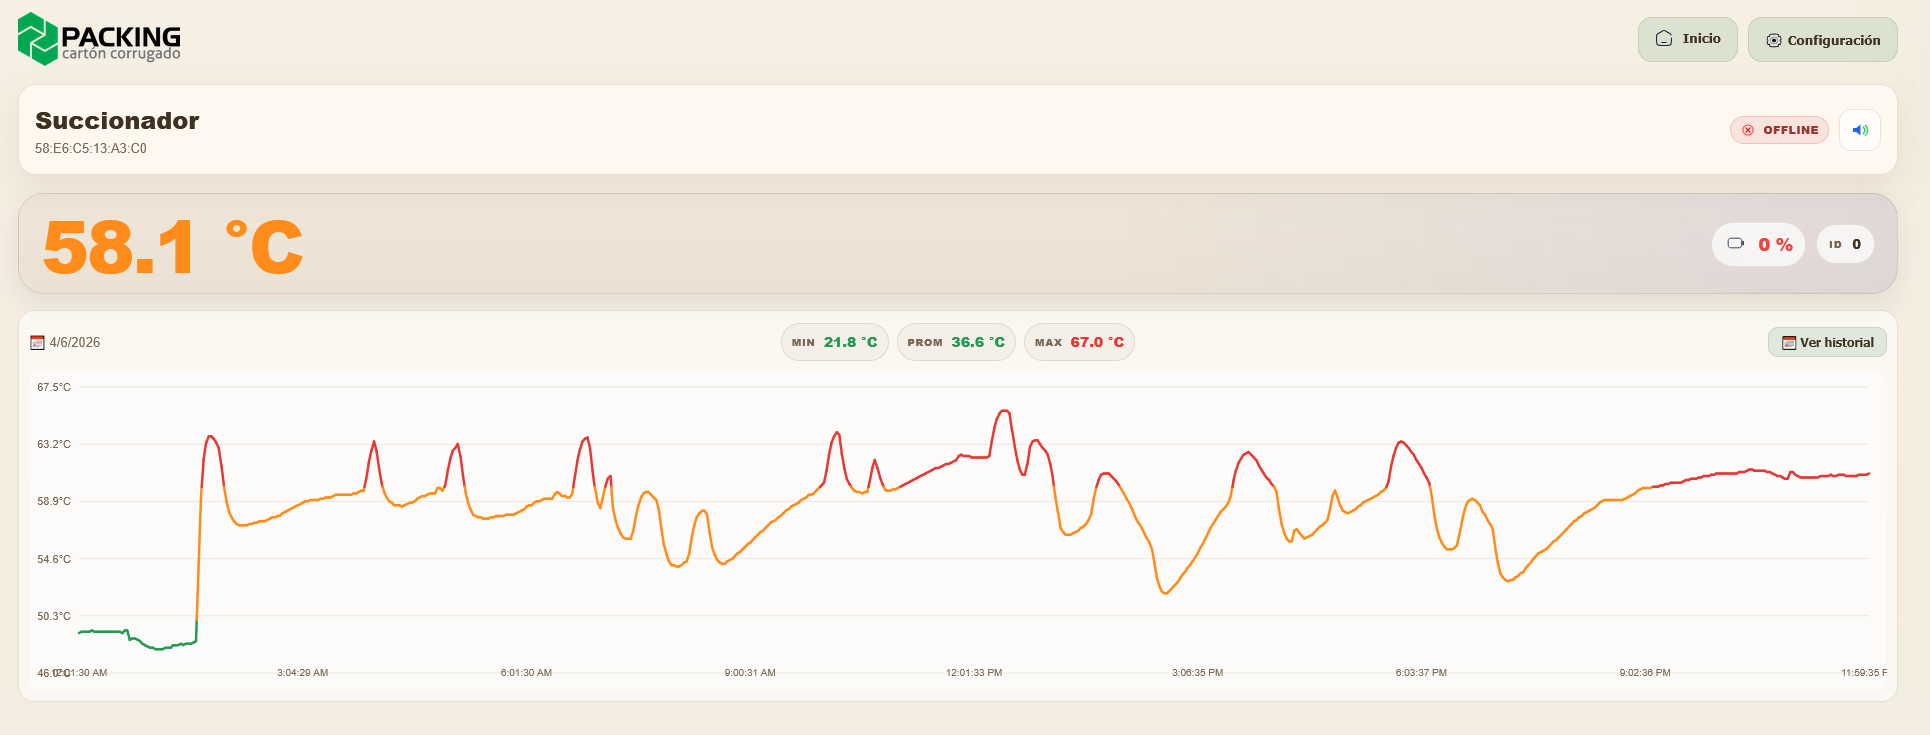
\includegraphics[width=\textwidth]{historico-succionador.png}
  \caption{Histórico térmico de 24 horas del succionador de la máquina Twin. La captura fue obtenida del dashboard local desarrollado. El estado \textit{offline} corresponde al momento de consulta del histórico y no invalida las muestras almacenadas.}
  \label{fig:historico-succionador}
\end{figure*}

La captura muestra un mínimo de \SI{21.8}{\celsius}, un promedio de \SI{36.6}{\celsius} y un máximo de \SI{67.0}{\celsius}. Sin embargo, los dos primeros valores no concuerdan con el intervalo visible de la curva. La revisión del dashboard mostró que la actualización periódica puede sobrescribir los indicadores del histórico seleccionado con las estadísticas del día actual, mientras conserva en pantalla la curva de la fecha consultada. Por rigor experimental, el mínimo y el promedio de esta jornada se recalcularán a partir del archivo original antes de utilizarlos como resultados cuantitativos.

\evidencia{archivo original del día, horas de marcha y parada de la Twin y confirmación de la inspección de rodamientos.}

\section{Evidencias complementarias pendientes}

La Fig.~\ref{fig:evidencias-pendientes} reserva los espacios de las evidencias que se incorporarán en la versión final. Cada fotografía deberá acompañarse con fecha, equipo, instrumento y una descripción breve del procedimiento realizado.

\begin{figure*}[!t]
\centering
\begin{minipage}[t]{0.24\textwidth}\centering
  \imgslot{Nodo PT100 instalado en el succionador de la Twin}\\[-1mm]
  {\footnotesize(a) Instalación del nodo}
\end{minipage}\hfill
\begin{minipage}[t]{0.24\textwidth}\centering
  \imgslot{Medición simultánea con pistola Fluke}\\[-1mm]
  {\footnotesize(b) Referencia Fluke}
\end{minipage}\hfill
\begin{minipage}[t]{0.24\textwidth}\centering
  \imgslot{Captura o fotografía de la cámara termográfica}\\[-1mm]
  {\footnotesize(c) Cámara termográfica}
\end{minipage}\hfill
\begin{minipage}[t]{0.24\textwidth}\centering
  \imgslot{Interfaz del Advantech WISE-2410 usada en planta}\\[-1mm]
  {\footnotesize(d) WISE-2410}
\end{minipage}

\vspace{2mm}

\begin{minipage}[t]{0.24\textwidth}\centering
  \imgslot{Tres nodos construidos y gateway con pantalla}\\[-1mm]
  {\footnotesize(e) Prototipos físicos}
\end{minipage}\hfill
\begin{minipage}[t]{0.24\textwidth}\centering
  \imgslot{Inspección o mantenimiento de los rodamientos}\\[-1mm]
  {\footnotesize(f) Evidencia mecánica}
\end{minipage}\hfill
\begin{minipage}[t]{0.24\textwidth}\centering
  \imgslot{Históricos de los otros puntos de medición}\\[-1mm]
  {\footnotesize(g) Otros sensores}
\end{minipage}\hfill
\begin{minipage}[t]{0.24\textwidth}\centering
  \imgslot{Configuración de offset y umbrales de alarma}\\[-1mm]
  {\footnotesize(h) Configuración}
\end{minipage}
\caption{Espacios reservados para las evidencias experimentales y de implementación que se incorporarán en la versión final.}
\label{fig:evidencias-pendientes}
\end{figure*}

\section{Discusión}

La principal ventaja evidenciada no fue únicamente la medición inalámbrica, sino la continuidad temporal. Un valor puntual informa el estado presente; una serie de tiempo permite identificar tendencias, retardos térmicos y eventos asociados con cambios de operación. El dashboard desarrollado facilitó este análisis al conservar el contexto diario completo.

La compensación configurable mejora la concordancia con una referencia, pero no reemplaza un procedimiento formal de calibración. La exactitud final depende de la clase de la PT100, la resistencia de los conductores, el contacto térmico, la ubicación de la sonda y la incertidumbre del instrumento de referencia. Por ello, la evaluación cuantitativa debe utilizar muestras simultáneas y documentar el montaje.

El límite actual de 30 días es una decisión de firmware y puede ampliarse según la capacidad de la microSD. Asimismo, los archivos poseen una estructura separada por comas, pero la versión revisada no expone todavía una ruta web de descarga CSV. Esta función debe verificarse en otra versión o implementarse antes de declararla como resultado definitivo.

\section{Conclusiones}

Se diseñó e implementó un sistema funcional para el monitoreo inalámbrico de temperatura superficial en una planta piloto. Los nodos adquirieron datos mediante PT100 de tres hilos y MAX31865, los transmitieron por LoRa y redujeron consumo mediante sueño profundo. El gateway almacenó las muestras y proporcionó visualización local sin depender de Internet.

El dashboard superó la presentación de un valor instantáneo al ofrecer históricos de 24 horas, estadísticas diarias, comparación entre sensores, compensación y alarmas configurables. Esta continuidad permitió observar un comportamiento térmico anómalo en el motor del succionador después de la parada de la máquina.

La comparación mostró que la pistola Fluke continúa siendo útil como instrumento de referencia puntual y que el WISE-2410 aporta variables industriales adicionales, especialmente vibración. SmartSense se destacó por la adaptación del dashboard a las necesidades específicas de visualización y análisis térmico de la planta.

Como trabajo siguiente se incorporarán las mediciones pareadas, se calculará el MAE antes y después de la compensación, se documentará la disponibilidad del enlace, se habilitará RSSI y se completará la exportación directa de datos.

\section*{Agradecimientos}

Los autores agradecen a la empresa aliada por facilitar el escenario de planta piloto, al profesor Jhon Edwin Vera por la dirección principal del proyecto y al profesor Sergio Francisco Mora Martínez por su acompañamiento durante la formulación y el desarrollo.

\begin{thebibliography}{99}

\bibitem{akyildiz2002}
I. F. Akyildiz, W. Su, Y. Sankarasubramaniam y E. Cayirci, ``Wireless sensor networks: A survey,'' \textit{Computer Networks}, vol. 38, no. 4, pp. 393--422, 2002.

\bibitem{yick2008}
J. Yick, B. Mukherjee y D. Ghosal, ``Wireless sensor network survey,'' \textit{Computer Networks}, vol. 52, no. 12, pp. 2292--2330, 2008.

\bibitem{centenaro2016}
M. Centenaro, L. Vangelista, A. Zanella y M. Zorzi, ``Long-range communications in unlicensed bands: The rising stars in the IoT and smart city scenarios,'' \textit{IEEE Wireless Communications}, vol. 23, no. 5, pp. 60--67, 2016.

\bibitem{semtech2015}
Semtech Corporation, ``AN1200.22 LoRa modulation basics,'' Application Note, 2015.

\bibitem{max31865}
Analog Devices, ``MAX31865 RTD-to-digital converter,'' Data Sheet, Rev. 3, 2015. [En línea]. Disponible: \url{https://www.analog.com/media/en/technical-documentation/data-sheets/MAX31865.pdf}

\bibitem{xiao}
Seeed Studio, ``Getting started with Seeed Studio XIAO ESP32-C6,'' 2026. [En línea]. Disponible: \url{https://wiki.seeedstudio.com/xiao_esp32c6_getting_started/}

\bibitem{ebyte}
Chengdu Ebyte Electronic Technology Co., Ltd., ``E220 series LoRa UART module user manual,'' documentación técnica del fabricante.

\bibitem{wise2410}
Advantech Co., Ltd., ``WISE-2410 LoRaWAN wireless condition monitoring sensor,'' Data Sheet, 2024. [En línea]. Disponible: \url{https://advdownload.advantech.com/productfile/PIS/WISE-2410/file/WISE-2410_DS(102324)20241023133301.pdf}

\bibitem{lee2015}
J. Lee, B. Bagheri y H.-A. Kao, ``A cyber-physical systems architecture for Industry 4.0-based manufacturing systems,'' \textit{Manufacturing Letters}, vol. 3, pp. 18--23, 2015.

\bibitem{shi2016}
W. Shi, J. Cao, Q. Zhang, Y. Li y L. Xu, ``Edge computing: Vision and challenges,'' \textit{IEEE Internet of Things Journal}, vol. 3, no. 5, pp. 637--646, 2016.

\end{thebibliography}

\end{document}
